\section{General description}
\label{sec:framework}

REST-for-Physics is composed of a set of libraries written in C++ and it is fully integrated with ROOT~\cite{ROOT,Brun:2011Gp,ROOT2011}, i.e. most C++ classes inherit from a ROOT TObject and therefore they can be read, accessed or written using the ROOT I/O interface. The only structural dependence is related to ROOT libraries, while other packages, as Geant4~\cite{Agostinelli:2002hh} or Garfield++~\cite{Garfield}, can be optionally integrated and used within the REST-for-Physics framework when generating or processing Monte Carlo data. Since REST-for-Physics is a natural extension of ROOT, we follow the same naming conventions, the Taligent rules. On top of those standard naming conventions, any REST-for-Physics C++ class (object) will always start with the \emph{TRest} prefix. In this paper we will highlight the words when they clearly make a reference to an existing REST-for-Physics C++ object: an object named \emph{TRestEvent} will be written as \emph{event} and an object named \emph{TRestAnalysisTree} will be written as \emph{analysis tree}. Therefore, a highlighted word, within context, expresses a deep connection with the different elements of the code.

%%%%%% THE MAIN FRAMEWORK DESCRIPTION %%%%%%%
\subsection{The REST-for-Physics framework}
Inside the REST-for-Physics ecosystem we distinguish a core library, or framework, that prototypes and fixes the implementation of most of the REST-for-Physics elements. Those base objects serve to define common methods and data members for specific\footnote{The reader should note that when we refer to specific objects, we refer to objects which inherit, in the strict sense of C++ object inheritance, from the base abstract objects, \emph{event}, \emph{metadata} and \emph{event process}. In the text, we will highlight the keyword \emph{specific} to refer to those inherited objects in a generic way, i.e. \emph{specific event} will be connected to any \emph{TRestSpecificEvent} and \emph{specific event process} will be connected to any \emph{TRestSpecificProcess}. It is worth observing that the event and the process objects contain the \emph{event} and \emph{process} keywords in their class name, while metadata classes usually omit the use of the \emph{metadata} keyword. } objects (see Figure~\ref{fig:objects}). We shall briefly introduce those basic elements:

\begin{itemize}
    \item The \emph{event} object encapsulates any specific \emph{event} data inside REST. It defines common fields, such as timestamp or event id, and it prototypes common methods used for printing or drawing event information. A particular \emph{specific event} implementation defines a type, thus it is important to note that in what follows we will distinguish between the \emph{event} data as the explicit contents of a particular \emph{specific event}, and the \emph{event} type as the format, or structure, of the \emph{specific event}. A \emph{specific event} representation is typically a physical quantity that needs to be described in a physical coordinate space or physical time, as it can be the time signals registered by an electronics acquisition system, or the energy deposits distribution produced by a Geant4 simulation.
    
    \item A \emph{metadata} object may be used as a mere information container, storing relevant parameters, such as the description of a Geant4 simulation, i.e. the \emph{geant4} metadata object, or it might adopt the shape of a complex object definition that implements advanced methods, such as the construction of a \emph{detector readout}, or a \emph{magnetic field} volume including interpolation routines. Those advanced \emph{metadata} objects will be found in specialized libraries. Conceptually we understand by \emph{metadata} any information required to give meaning to any \emph{specific event} data. Therefore, any input or output parameters required during the processing or transformation of \emph{event} data, or type, using \emph{event processes}, is also regarded as \emph{metadata}. Any metadata class can be initialized through a XML configuration file.
    
    \item The \emph{event process} object defines an input/output \emph{event} protocol allowing to interconnect different \emph{specific event process} implementations into a sequential processing chain. This object will be able to perform operations with the input \emph{specific event} transforming its type and/or its contents, returning at the output \emph{specific event}. The \emph{event process} itself inherits from the \emph{metadata} object, since a process usually requires initialization to define input parameters that control the behavior of the process.
\end{itemize}

% This figure is available for edition here
% https://docs.google.com/presentation/d/14pQh7u6gqyeinPss1HClYSZ0S5690bLzObTaWKJaKzE/edit?usp=sharing
\begin{figure}[]
  \centering
  \raisebox{-0.5\height}{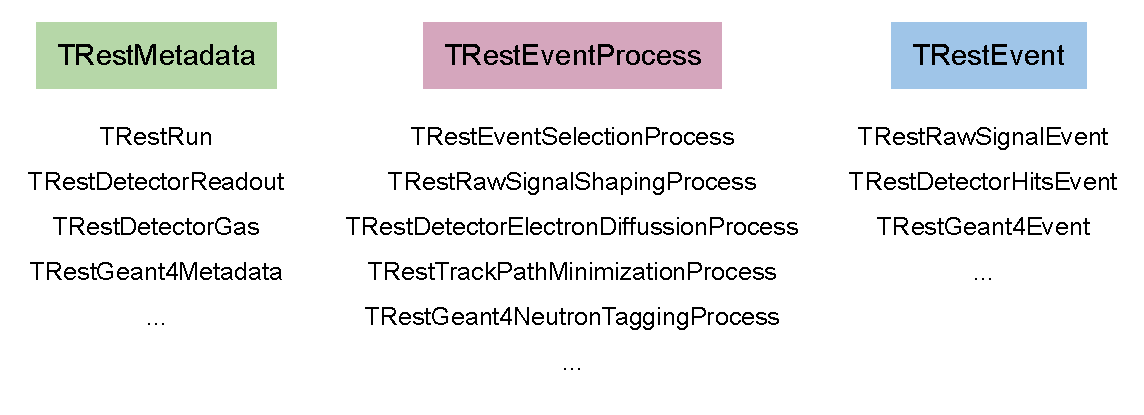
\includegraphics[trim=0 20 0 0, clip,width=0.95\linewidth]{images/RESTClassExamples.pdf}}
	\caption{The base REST-for-Physics framework objects, 
	\emph{metadata}, \emph{event process} and \emph{event} together with few examples of specific implementations.}  \label{fig:objects}
\end{figure}

We will find other elemental tools inside the main framework, such as string helper methods, fundamental physics constants and units system or other basic mathematical tools useful for the development of any specific \emph{event process}. Any \emph{metadata} or \emph{event process} object that does not require specific specialization will likely be hosted inside the framework domain.
 In addition, the framework repository\,\cite{REST_Framework_Git} centralizes other REST-for-Physics components, such as libraries or packages. Those components will be introduced in section\,\ref{sec:libraries}.%SUB-MODULES

% Describe sub-modules, libraries and packages.

% framework core, tools, analysis

% define \emph{metadata} to TRestMetadata naming convention

% Submodules, Libraries, packages, projects

%%%%%% I/O Access and storage %%%%%%%
\subsection{I/O access and metadata storage}

%% Paragraph dedicated to REST progress and philosophy % Description of metadata+data concept
%% During the last years, major upgrades took place on the REST core libraries\,\cite{Galan_8thTPC}. 


% TRestRun (any event data processing taking place with REST will write to disk a TRestRun object, any REST object taking active part on the data processing will be stored in ROOT file.
REST-for-Physics uses the ROOT I/O interface to write \emph{event} and \emph{metadata} objects to disk. A ROOT file generated with REST may contain any number of \emph{specific event} and \emph{specific metadata} objects, including any \emph{specific event process} (being a \emph{metadata} object itself). Those objects are stored in a unique file, together with the \emph{run} metadata object and the \emph{analysis tree} that are always present in any file that has been processed with REST (see Figure~\ref{fig:file_contents}). The \emph{run} object registers values to identify the data file and the conditions the data were registered, such as the start time, duration, run number, etc, while the \emph{analysis tree} collects per event information, named observables, at any stage of the data processing. The \emph{run} object takes also an active role when accessing the different objects stored on disk by implementing helper methods to access the data; for example, getting a list of events fulfilling particular conditions at the \emph{analysis tree} or retrieving directly the pointer to a given event id number, and updating simultaneously its corresponding \emph{analysis tree} entry.

\begin{figure}[tb]
  \centering
  \raisebox{-0.5\height}{
 
  %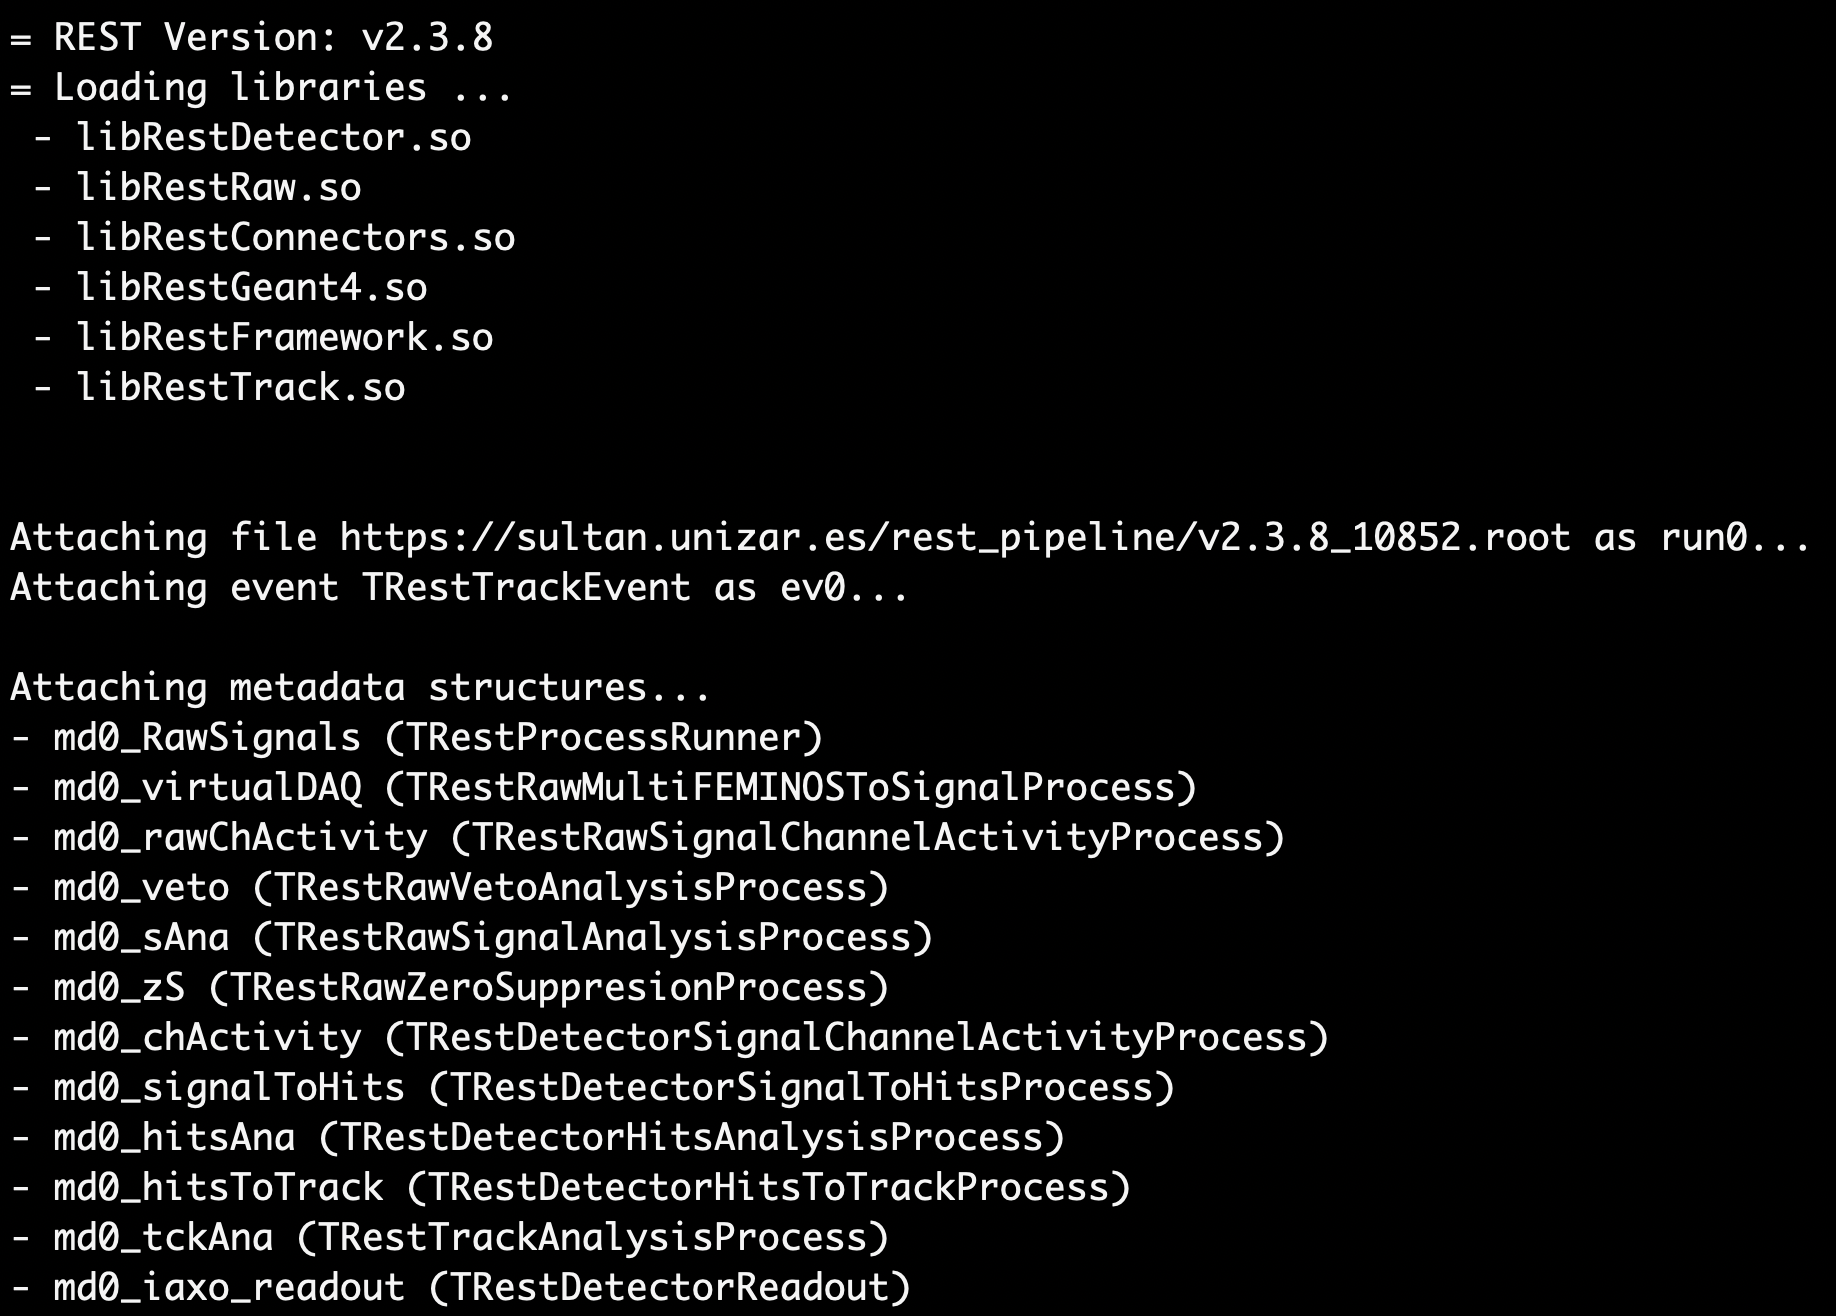
\includegraphics[width=0.68\linewidth,trim=0 0 10 0, clip]{images/REST_file_contents_restRoot.png}
  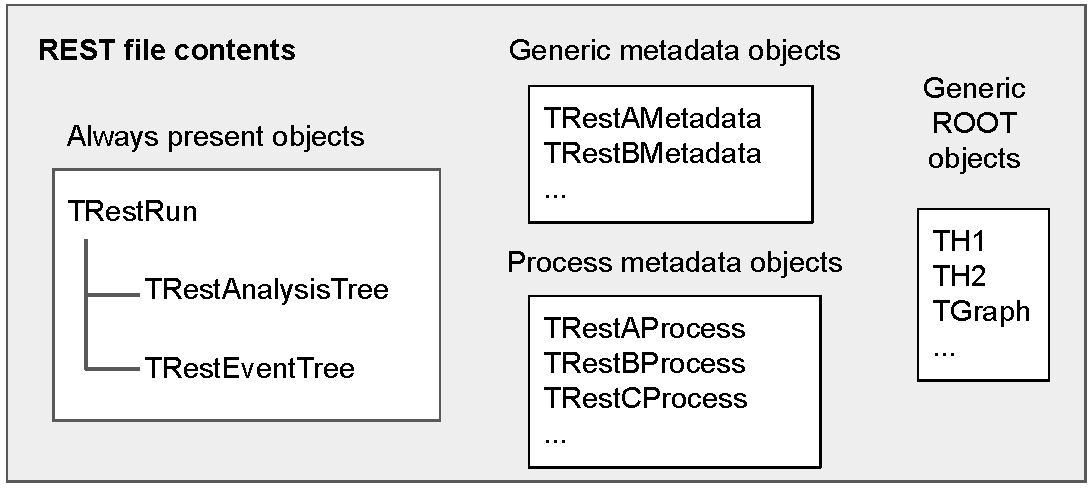
\includegraphics[width=0.75\linewidth,trim=0 0 0 0,clip]{images/RESTFileContents.pdf}
  }
	\caption{A schema showing the different components that may be present inside a REST data file. The \emph{analysis tree} and \emph{event tree} objects are independent objects accessed through the \emph{run} interface which ensures coherent access to a particular event entry linked to its corresponding analysis entry.} \label{fig:file_contents}
\end{figure}

% something about metadata
The framework philosophy is to create \emph{specific metadata} objects with dedicated data members to store any information crucial for the final analysis, and/or to fully determine the nature of the data we are storing. All the \emph{metadata} inherited objects gain data member reflection support, thus creating a relation between the C++ conceptual class members and the text fields used in the configuration files. Through the implementation of the \emph{metadata} object we have designed a dedicated configuration file format for REST, based on Extensible Markup Language (XML). This upgrade allows the reading of XML files with additional features, such as system environment variables, complex programming instructions, including \emph{if} conditions or \emph{loops}, evaluation of mathematical expressions or even support for arbitrary physical units conversion inside any parameter. We assign a new extension, \emph{rml}, to this upgraded XML format.

Using the \emph{metadata} philosophy we create a unique relation between the configuration files and the C++ objects. One XML element is identified with one \emph{metadata} object, with its attributes associated to the data members inside the object. If there is an embedded element inside the XML element, it is associated in-chain to the corresponding \emph{metadata} member. In this way, the automatic initialization of \emph{metadata} objects is achieved, without any file reading methods in the class.

\subsection{Event data processing and analysis}

The framework allows to build an event data processing chain in a modular way by interconnecting already existing \emph{specific event processes}, or developing new ones with the potential to plug them directly to an existing processing chain. Each \emph{event process} has access to the input \emph{specific event}, the \emph{analysis tree} and any \emph{metadata} object that is accessible by the \emph{run} object. Depending on the input/output \emph{specific event} interaction inside the process, we may attempt to classify the \emph{event processes} into different groups, as illustrated in Figure\,\ref{fig:dataChain}:

\begin{itemize}
\item An \emph{external process} is a process that reads an external data source, usually at the beginning of a REST processing chain. It might be binary data generated by an acquisition system, or Monte Carlo data generated by an external simulation package. The process will be in charge of understanding the format of that external data serving to initialize a REST \emph{specific event}.

\item An \emph{internal transformation process} is a process in which the \emph{specific event} input is the same type as the \emph{specific event} output. The \emph{event} data will be transformed but not the \emph{event} type.

\item A \emph{pure analysis process} accesses the information of a \emph{specific event} type and produces observables that will be added to the \emph{analysis tree} but it will not modify the \emph{specific event} contents in any sense. A pure analysis process might serve, for example, to implement a complex physics model that uses the \emph{specific metadata} and \emph{specific event} information to elaborate some results that will be exported to the \emph{analysis tree}, or a \emph{specific metadata} object.

\item A \emph{general process} is a process that does not access the information inside the \emph{specific event} type. It will only need access to the basic \emph{event} information common to all \emph{specific events}, and/or the \emph{analysis tree}. Therefore, this process may be plugged at any point of a data processing chain without restrictions. Processes of this kind may have many different purposes as it could be; to visualize online \emph{analysis tree} observables on real time, implement a \emph{summary} process to calculate averages (or any other statistical variable) from the \emph{analysis tree}, or perform a generic fitting of a variable at the \emph{analysis tree} spectra placing the fitting results at a dedicated metadata object, among many other basic analysis tasks.

\item A \emph{transformation process} is a process that receives as input a \emph{specific event} and transforms it to a different \emph{event} type. This kind of processes will all be placed at the \emph{connectors} library, described in section\,\ref{sec:libraries}, in order to encapsulate all library inter-dependencies in a single entity. 
\end{itemize}

%% This figure is available here: https://docs.google.com/presentation/d/1a2gdqvANFdbIq_GCrF9XQyBjAOBtZc5N9xahquPdVpE/edit?usp=sharing
\begin{figure}[tb]
  \centering
  \raisebox{-0.5\height}{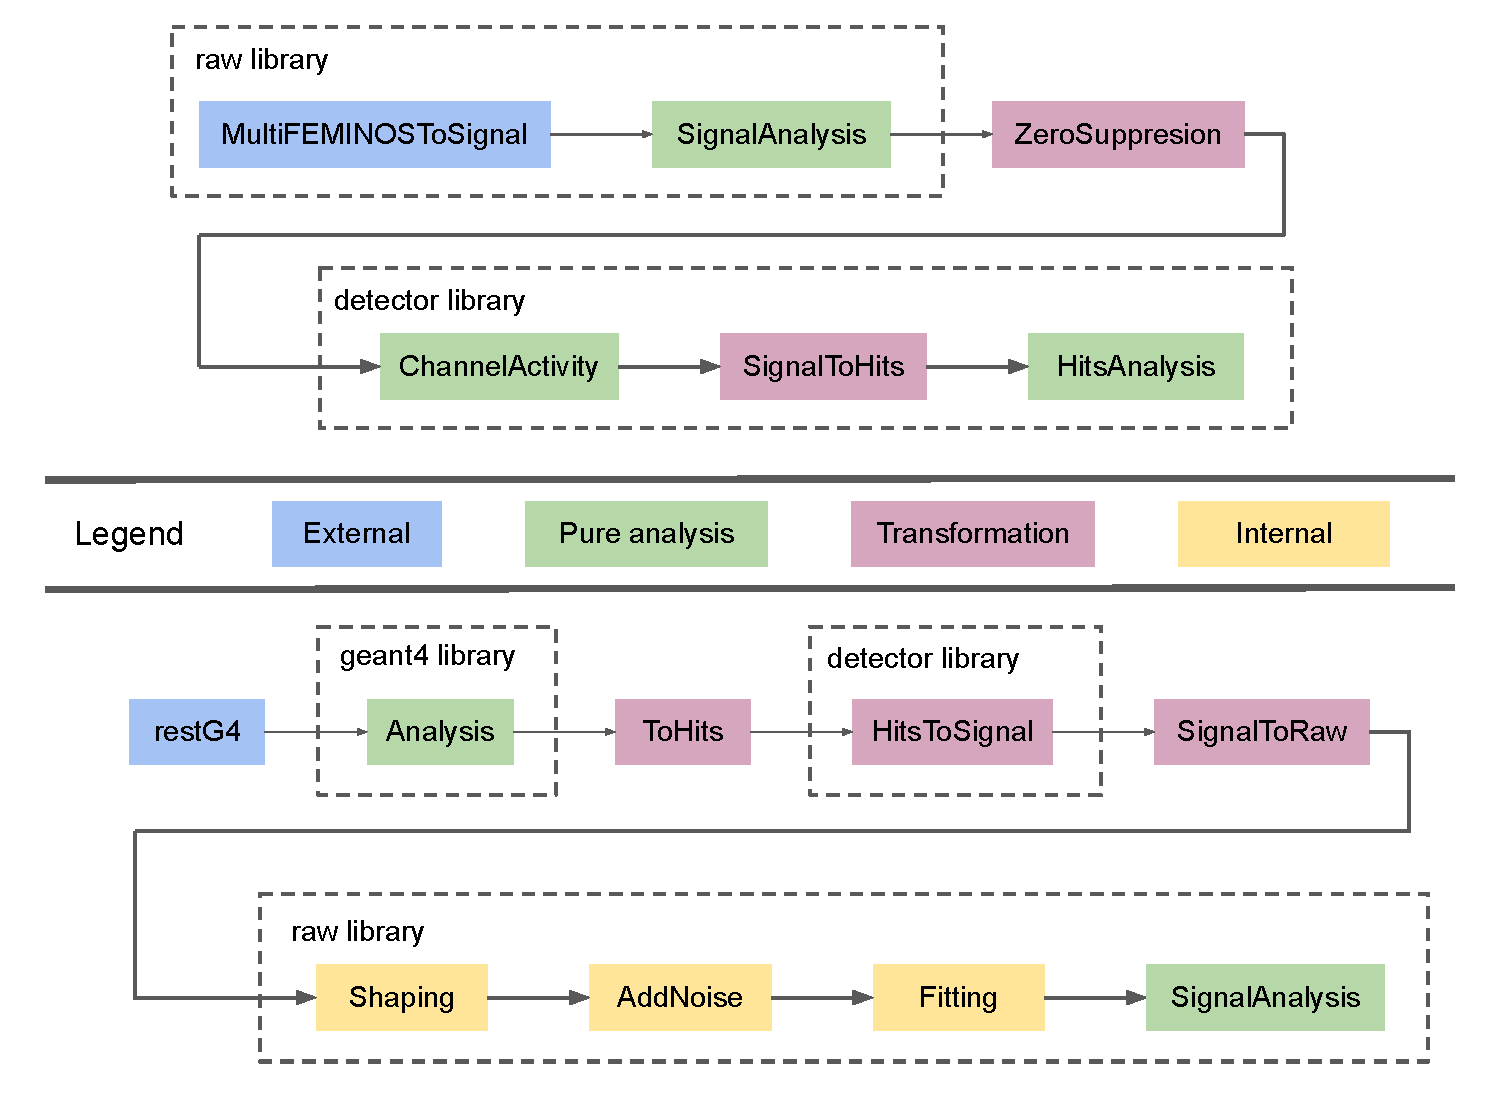
\includegraphics[width=0.95\linewidth]{images/DataChain.pdf}}
	\caption{A schema showing the event data flow for two different data chain implementations in order to illustrate the different processes classification (using a color legend). On the \emph{top}, an experimental detector data processing chain reading a binary file, analyzing, and post-processing the rawdata for event reconstruction. On the \emph{bottom}, a Monte Carlo generated data processing chain, where the data are analyzed and transformed to match the data format in a raw electronics acquisition system, where we condition the data using \emph{shaping}, \emph{add noise} and \emph{fitting} internal processes belonging to the raw library. We observe in this schema how different libraries (geant4, detector, raw) described on section\,\ref{sec:libraries} intervene at different stages, and how those play a role on both, Monte Carlo and experimental data.}  \label{fig:dataChain}
\end{figure}

% Event transformation
A \emph{specific event} might be transformed during the event processing and, in that transformation, relevant information might not be available anymore at the final transformed output event. The reason is that the role of the \emph{specific event} object is to provide a faithful or significant representation of the data at the state of processing where we are inside our processing chain: i.e. at different processing stages we might have the event data made of time signals registered at an electronics setup, or we might have the event data in the shape of discrete energy deposits at a physical coordinate system. Therefore, the transformation from one event data representation, or \emph{specific event}, into another, means that a relevant parameter available at a particular stage, is not available anymore.

% Analysis tree description
The \emph{analysis tree} comes into play as an instrument to collect all those parameters extracted or calculated from the \emph{specific event} information which will be relevant for the final analysis.  Any \emph{specific event process} in the processing chain is allowed to add new observables to the \emph{analysis tree}. Once a process adds an observable to the \emph{analysis tree}, this observable will always be available even if the \emph{event} data is transformed or the processing chain happens in several steps using different input/output REST data files. The information in the \emph{analysis tree} is always accumulative, and therefore it will contain a full summary of the observables added by each process (see Figure\,\ref{fig:observables}).


\begin{figure}[tb]
  \centering
  \raisebox{-0.5\height}{
  \begin{tabular}{c}
  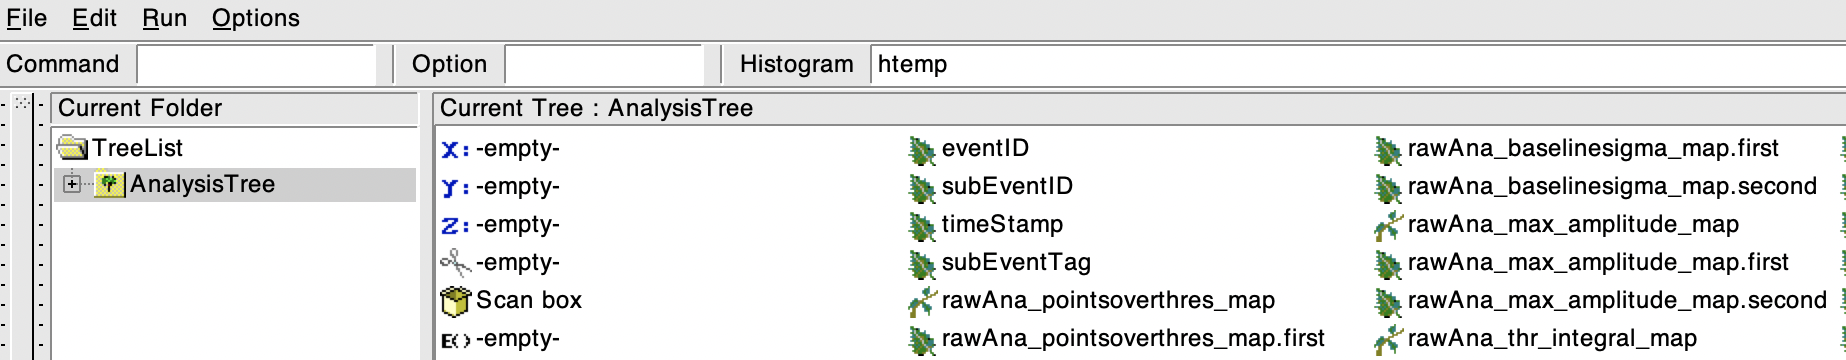
\includegraphics[width=0.98\linewidth,trim=0 0 10 0, clip]{images/TBrowser.png} \\
  
  \\
  
  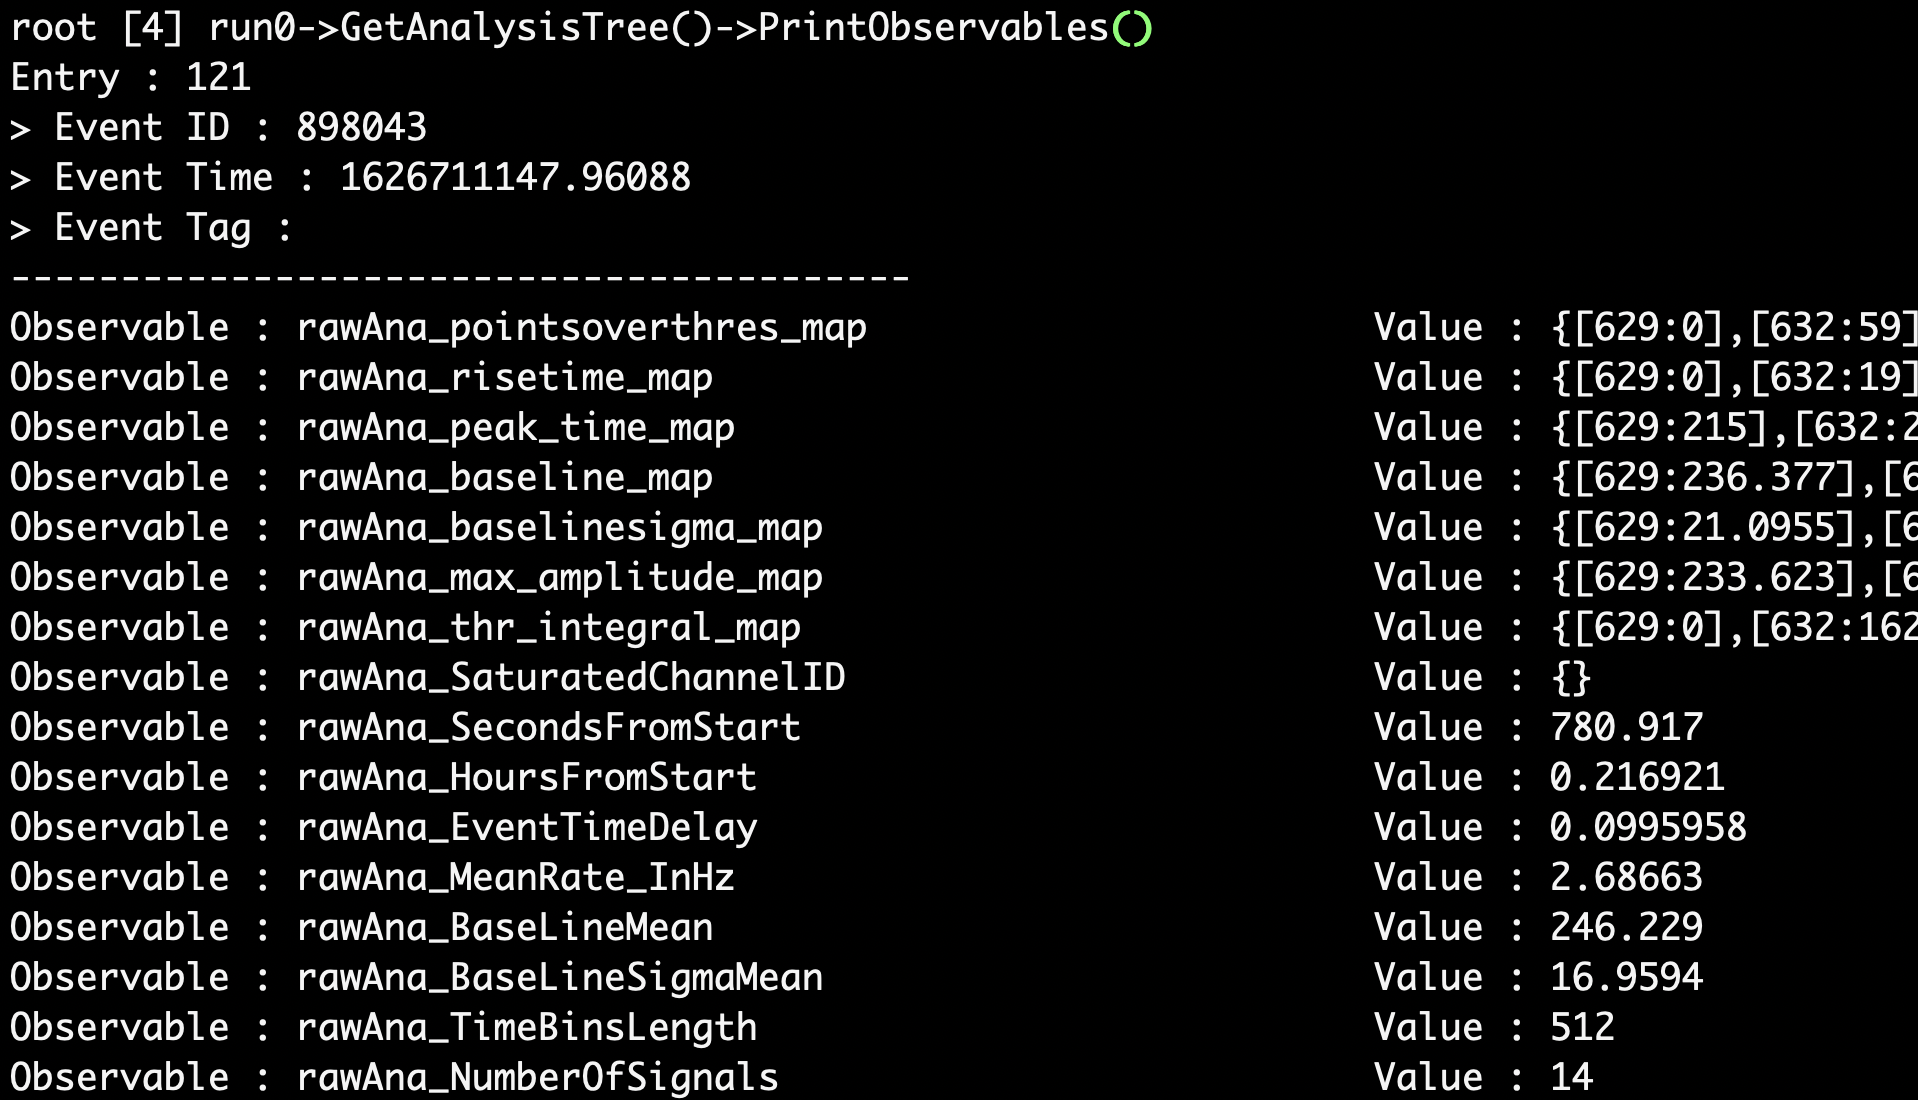
\includegraphics[width=0.65\linewidth,trim=0 98 0 0, clip]{images/observables.png} \\
  \end{tabular}
  }
	\caption{Two snapshots showing the observables registered at the analysis tree. At the \emph{top}, we inspect the observables using a ROOT \emph{browser} object. At the \emph{bottom}, we inspect the analysis observables at a particular event entry using the ROOT command line interface.}\label{fig:observables}
\end{figure}

In brief, the \emph{analysis tree} provides a way for \emph{specific event processes} to export an analysis result, extracted from each event, to the framework. It must be noted that the processes have two ways to export results, an event-per-event based observable inside the \emph{analysis tree}, or a given result common to all the events in a particular \emph{run}, that will be exported in the form of a \emph{specific metadata} object.

The information extracted by a process and added to the \emph{analysis tree} might be as simple as just a registered value available at the \emph{specific event} at a given stage of the processing chain, or it might be the result of a complex calculation in the context of a physics model, including complicated input \emph{metadata} objects or parameters. Of course, even in the case of basic observables extracted directly from the \emph{specific event}, the user might be interested to know the evolution of such observable after an intermediate processing. In order to do that, it is possible to define the same \emph{specific event process} at different positions in the sequential processing chain.

%defines a particular analysis job upon a particular input event in order to manipulate the \emph{specific event} data, transform it and extract relevant information. 

%Afterwards the \emph{event process} must yield an output event. 

%In principle, any \emph{event process} that participates in a data processing chain must satisfy that its input event type corresponds with the output event type of the previous \emph{event process}. 

The \emph{event process} object implements a method to facilitate the addition of observables to the \emph{analysis tree}. This method allows to directly create or set the value for an observable from any C++ variable (supporting various C++ types, from base types to proper \emph{stl} containers, and either global or local variables). This method simplifies the coding of REST \emph{event processes} by avoiding users to directly interface the \emph{branch} and \emph{tree} ROOT objects, and at the same time it is used to encapsulate common naming conventions for observable names, or other analysis REST standard definitions.

%% discuss how to analyze Monte Carlo and experimental data using common event processes
Our framework design is completely transparent to the processing of real experimental data, or Monte Carlo simulated data. The reason is that a \emph{specific event process} implementation may operate on both scenarios. The only requirement is that the experimental or simulated input \emph{event} must be given to the process in the form of a \emph{specific event} type. If both, simulation or experimental data, are conditioned to fit in a common \emph{specific event} type, we will be able to build a processing chain that not only processes simulated data or experimental data, but that fully combines both. As a hypothetical case, we could integrate a process simulating the signal shaping of electronics into real experimental data to assess the benefit of applying such electronics setup in our real experiment. Furthermore, a proper conditioning of the generated Monte Carlo \emph{event} data will allow the evaluation of the algorithms for analysis to be used with the real experimental data even before the start of the physics data taking program.

%% discussion about multi thread 
Event processes are executed through an efficient engine, or \emph{process runner}, with multi-thread support. The data processing chain is cloned into multiple instances and kept in different threads respectively. During execution, the input event is in turn dispatched to each thread for processing, while the output event is redirected to the global output file for writing, leading to an increase of processing speed proportional to the number of threads enabled. Figure\,\ref{fig:processing} summarizes the input/output processing logic and the different concepts already described in this section.   %Multi-thread operation is most helpful in case of algorithm verification, for example we can quickly get the result of a newly added observable to see if the code is alright.

\begin{figure}[htb!]
  \centering
  \raisebox{-0.5\height}{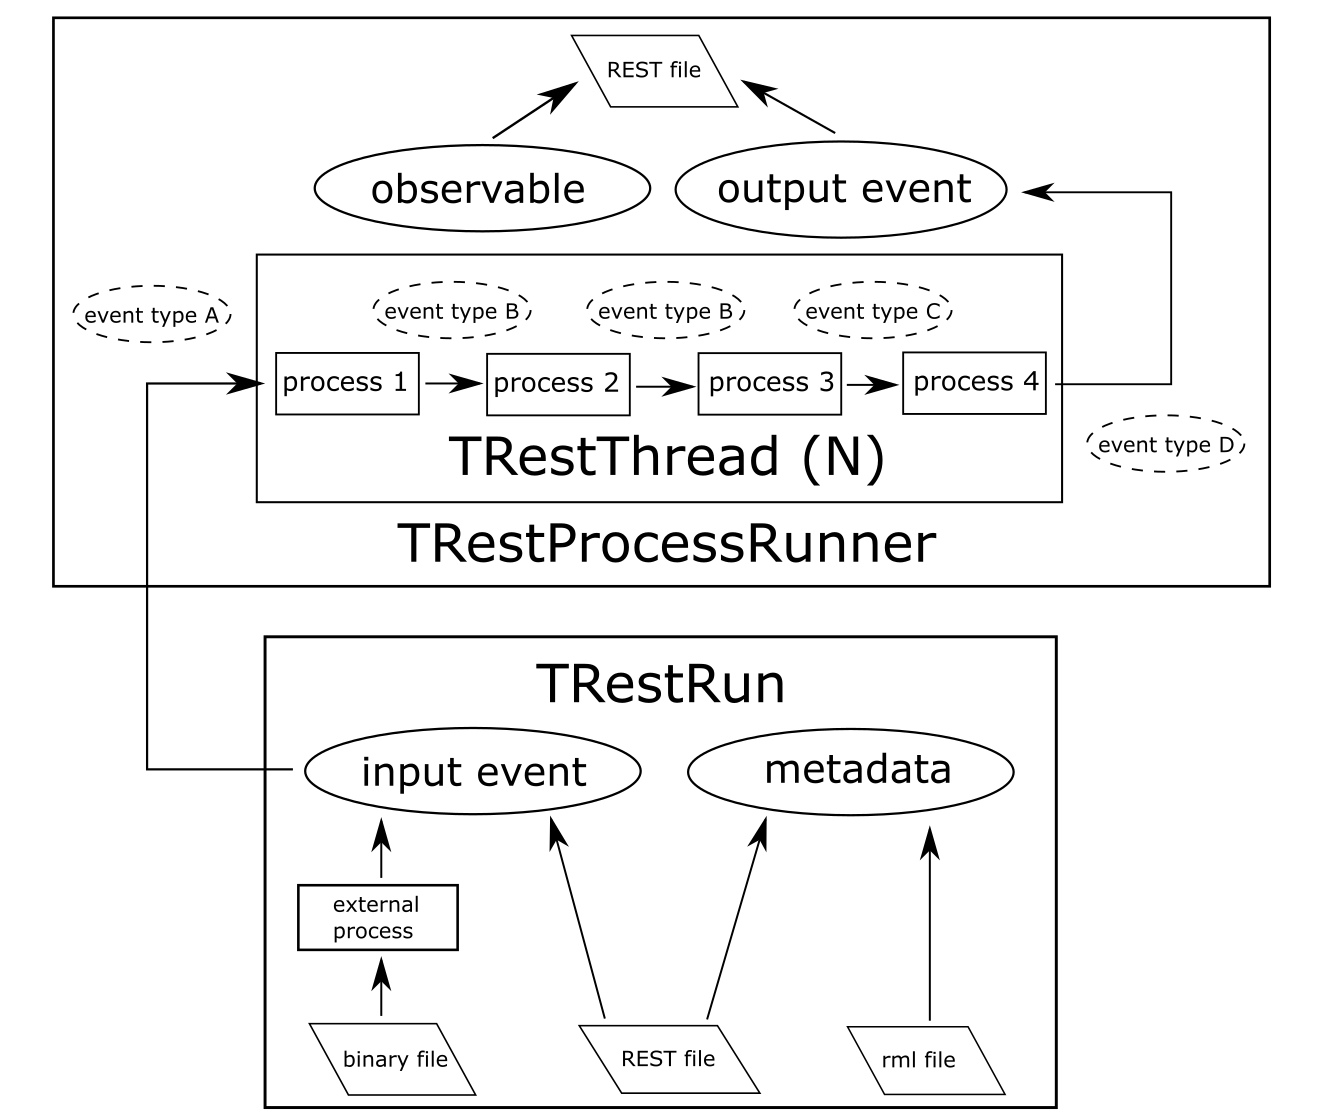
\includegraphics[width=\linewidth]{images/process_chain.png}}
	\caption{A schematic diagram showing the event data flow inside a REST processing chain. The \emph{run} object is initialized, and it has access to any \emph{specific metadata} or \emph{event} data available at the input REST file, or any additional objects described through \emph{rml}. The data is then processed using the implementation inside the \emph{process runner} object. Different event types (A,B,C,D) make reference to different \emph{specific event} implementations. The resulting output REST file will contain all the \emph{metadata} information available to the chain, including any previously available, together with the transformed output \emph{specific event}, and the updated \emph{analysis tree}.  }\label{fig:processing}
\end{figure}

\subsection{Visualization and plotting}

REST-for-Physics implements routines for event visualization and observable plotting based on ROOT drawing objects and methods. We use ROOT graphical interface objects to create basic tools, such as an \emph{event browser} with a control panel and a drawing pad (see Figure\,\ref{fig:eventBrowser}). The drawing pad itself is the target of the \emph{draw event} method implemented at each \emph{specific event}. If enabled, different output \emph{specific event} trees - from different stages at the data processing - will be stored in the same file. In that case the \emph{event browser} will be able to switch between the different event data representations.

\begin{figure}[h]
  \centering
  \raisebox{-0.5\height}{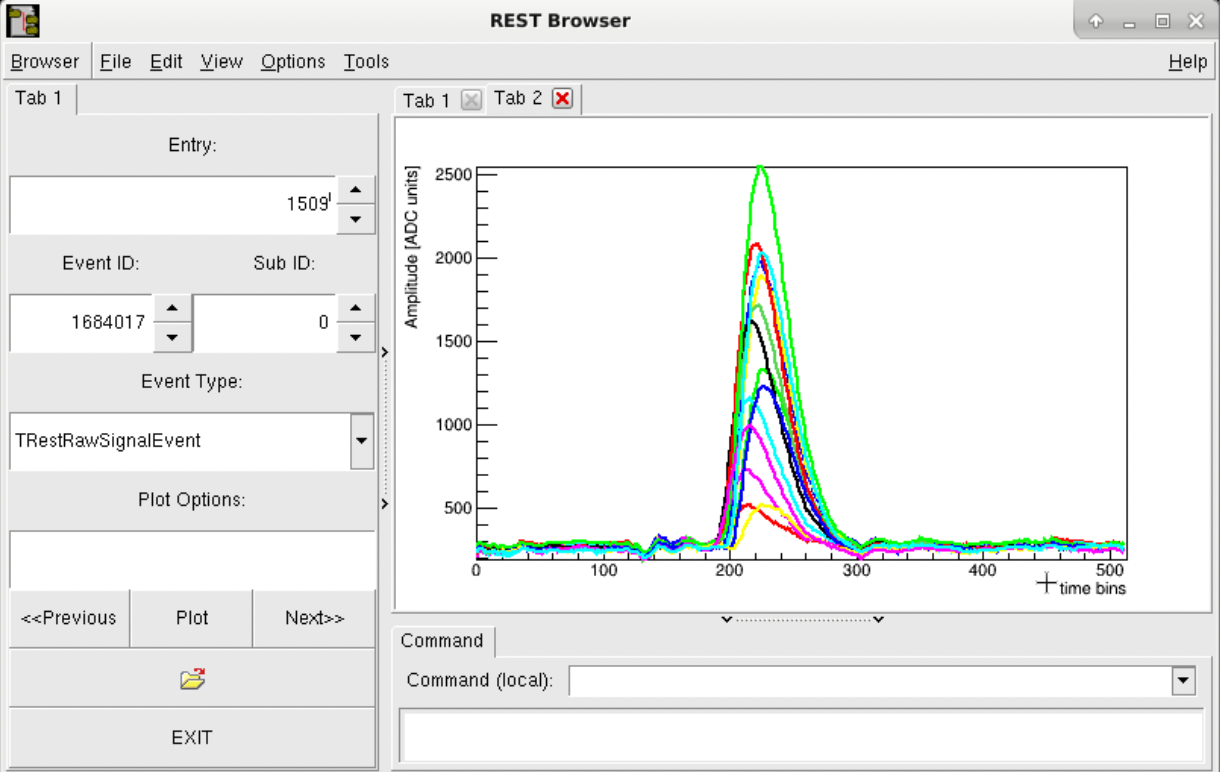
\includegraphics[width=0.45\linewidth]{images/EventBrowser.png}\,\,\,\,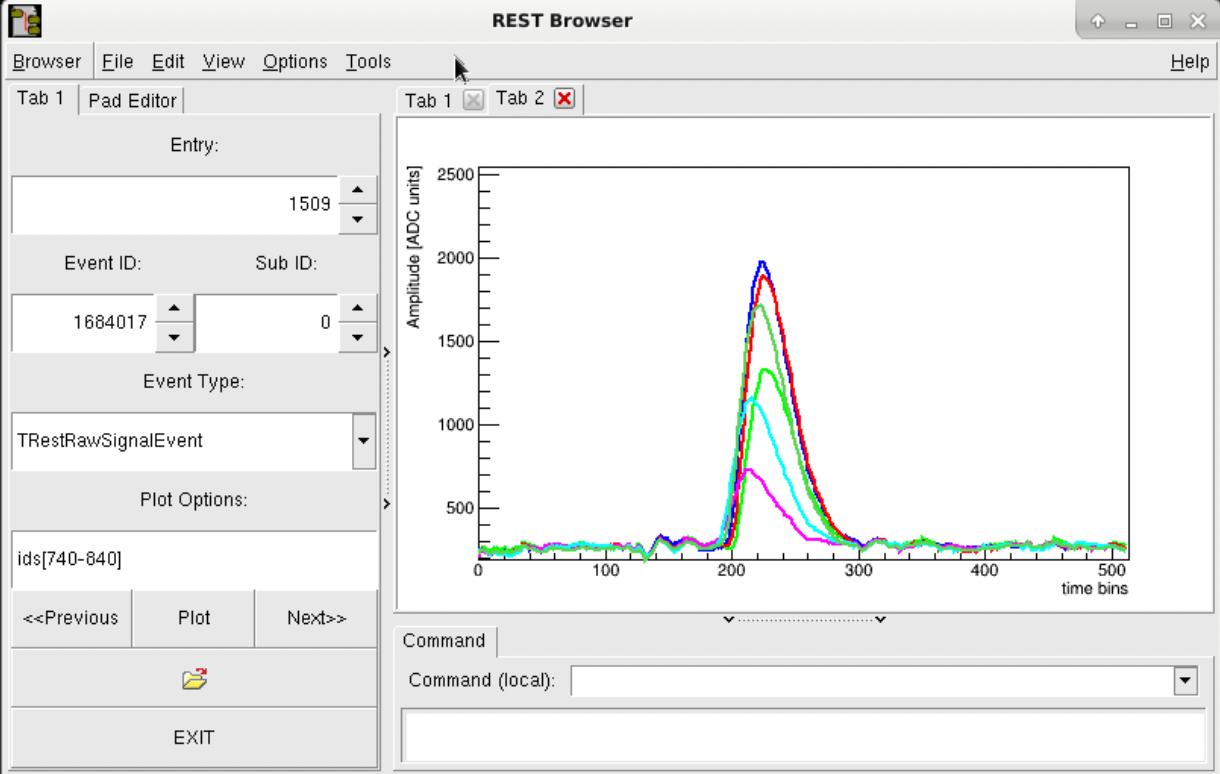
\includegraphics[width=0.45\linewidth]{images/EventBrowserSelection.png}}
	\caption{Two snapshots from the REST \emph{event browser} where we observe the control panel and the drawing pad showing an event entry for a \emph{raw signal event} (see section\,\ref{sec:libraries} for details on the \emph{specific event} type). On the left figure we present the complete event, while on the right figure the pulses have been filtered using an option passed to \emph{draw event} method implemented at each \emph{specific event}.}\label{fig:eventBrowser}
\end{figure}

%%%%%%%%%%%%%%%%%%%%%%%%%%%%%%%%%%%%%%%%%%%%%%%%%%%%%%%%%%%%%%%%%%%%%%%
%% This is true, we have the choice to put all them together. But it would be good to implement a kind of "smart" event browser that would open all the previous files used on the processing and contain event data. Then we would create a new TAB for each type on the window PAD, there where it says "TAB 1", "TAB 2".
%%%%%%%%%%%%%%%%%%%%%%%%%%%%%%%%%%%%%%%%%%%%%%%%%%%%%%%%%%%%%%%%%%%%%%%
%% THIS IS AN OPTION
%As described above, multiple event branches are stored in REST output file corresponding to the different stages of data processing. Each type of \emph{event data} contains a default visualization method to be drawn on the pad. When opening the file for visualization, one can simply switch between the entries, and view the \emph{event data} at different stages.
%%%%%%%%%%%%%%%%%%%%%%%%%%%%%%%%%%%%%%%%%%%%%%%%%%%%%%%%%%%%%%%%%%%%%%%

The \emph{analysis tree} object inherits directly from a ROOT \emph{tree} object, and therefore we may exploit all the resources provided by ROOT when analysing the observables that have been added to the \emph{analysis tree} by the different \emph{specific event processes} at the processing chain: i.e. we can use a ROOT \emph{browser} to explore the REST data files, and quickly draw and inspect variables from the \emph{analysis tree} (as shown previously in Figure~\ref{fig:observables}).

Furthermore, REST implements dedicated tools for automatic and systematic plot generation, such as the \emph{analysis plot} or the \emph{metadata plot} objects. 
The \emph{analysis plot} will efficiently integrate the capability to merge thousands of files through an \emph{rml} file in which the desired plots with the combined data will be defined, including advanced features such as classifying the produced histograms as a function of any \emph{specific metadata} member stored in the files, or define selection criteria based on the \emph{analysis tree} observables that serve to filter the data to be plotted. The \emph{analysis plot} object allows the creation of a plot definition that can be used, for example, to produce quick analysis reports in \emph{pdf} format (see Figure~\ref{fig:quickAna}) or to export histogram data in any other file format supported by ROOT.
The \emph{metadata plot} object allows to read many REST generated files and draw any \emph{specific metadata} member as a function of another \emph{specific metadata} member extracted from each of the REST files provided. This enables the study of; the correlation between any two metadata parameters, or the evolution of a metadata parameter as a function of the \emph{run} time, or the associated run number, for example.

\begin{figure}[h]
  \centering
  \raisebox{-0.5\height}{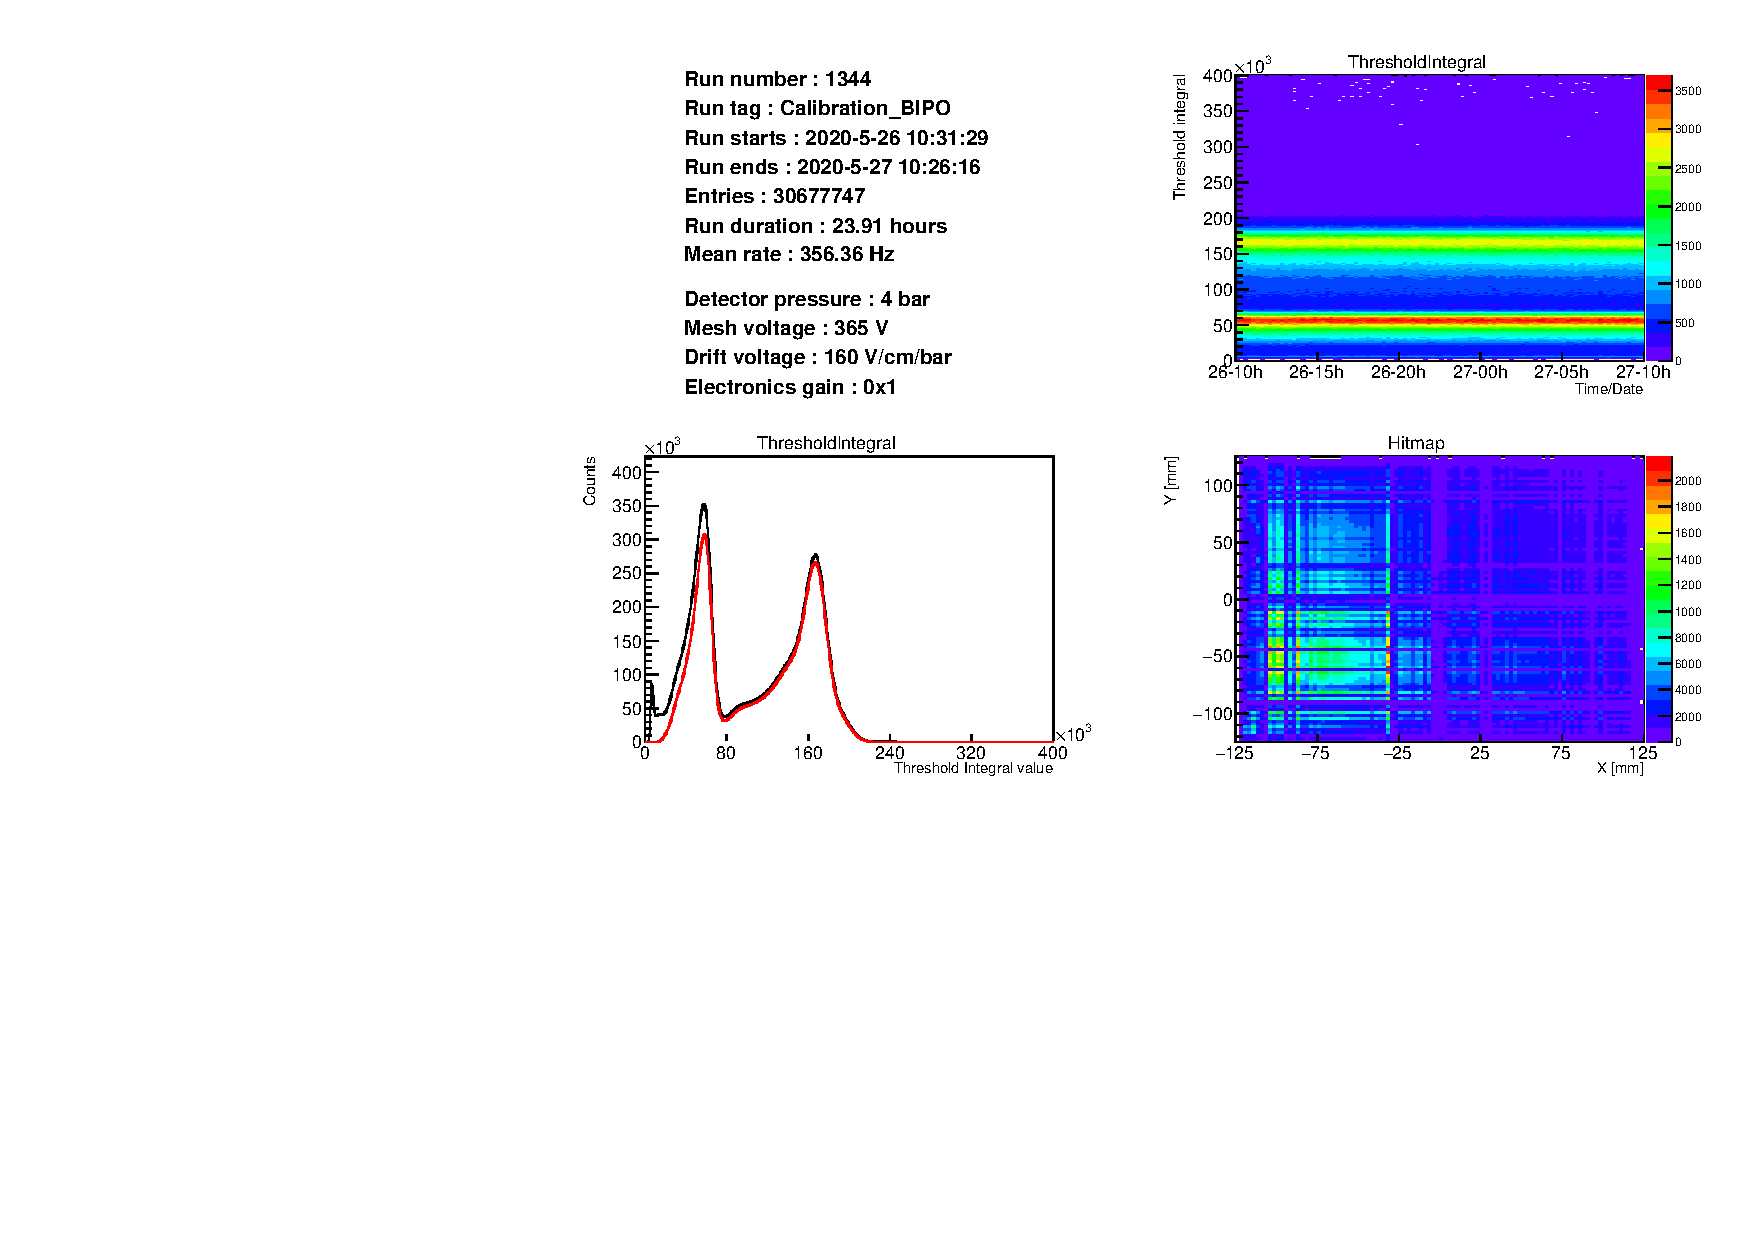
\includegraphics[width=0.9\linewidth]{images/TREXDM_Summary.pdf}}
	\caption{A summary report produced by the quick analysis system integrated at TREX-DM using REST. The plots are generated using \emph{analysis tree} observables. We observe a panel with \emph{run} details and other \emph{specific metadata} information (top-left), an energy spectrum (bottom-left), an energy spectra evolution along the run duration (top-right) and a distribution of the mean positions, or hitmap, where the event interactions took place (bottom-right). The \emph{ThresholdIntegral} is an observable produced by the raw library that represents the detected energy.}
	\label{fig:executables}
\end{figure}

%Histograms of \emph{observables} are generated with REST's analysis plot logic. Pads, plots, axis, legends, or even sub-pads and sub-plots, can all be defined through our \emph{rml} configuration file, ensuring better hierarchy and readability than C++ codes. Multiple files can be merged to a single figure or be classified into different figures. Figures can be drawn into pdf files with a single command. 

% TRestAnalysisPlot, TRestMetadataPlot, ...

\subsection{Execution and job management}
% restRoot, macros, practical data chain processing definition
Two executables are provided at the top level of the REST-for-Physics framework and are always available to any REST user, \emph{restRoot} and \emph{restManager}: the former provides a ROOT interactive prompt with REST libraries loaded, and optionally, with all the available REST macros preloaded; \emph{restManager} manages the execution of jobs. It may launch a processing chain defined through the \emph{process runner}, execute a method defined at any REST object available to the \emph{run} object or launch a ROOT C++ macro file. 

ROOT C-macros can be used to execute very specific but common tasks accessing the information inside REST data files. Official REST macros distributed with the framework may have been assigned an alias to facilitate its execution at the command line. Packages, or applications, that link to REST libraries will also provide their own executables, such as \emph{restG4} or \emph{restFileIndexer}  (see Figure~\ref{fig:executables}). \emph{restManager} allows the definition of all those actions through a configurable \emph{rml} file, but the \emph{manager}, executed through the \emph{restManager} executable, guarantees that the event data processing flow follows the standards previously described in Figure~\ref{fig:processing}.

\begin{figure}[h]
  \centering
  \raisebox{-0.5\height}{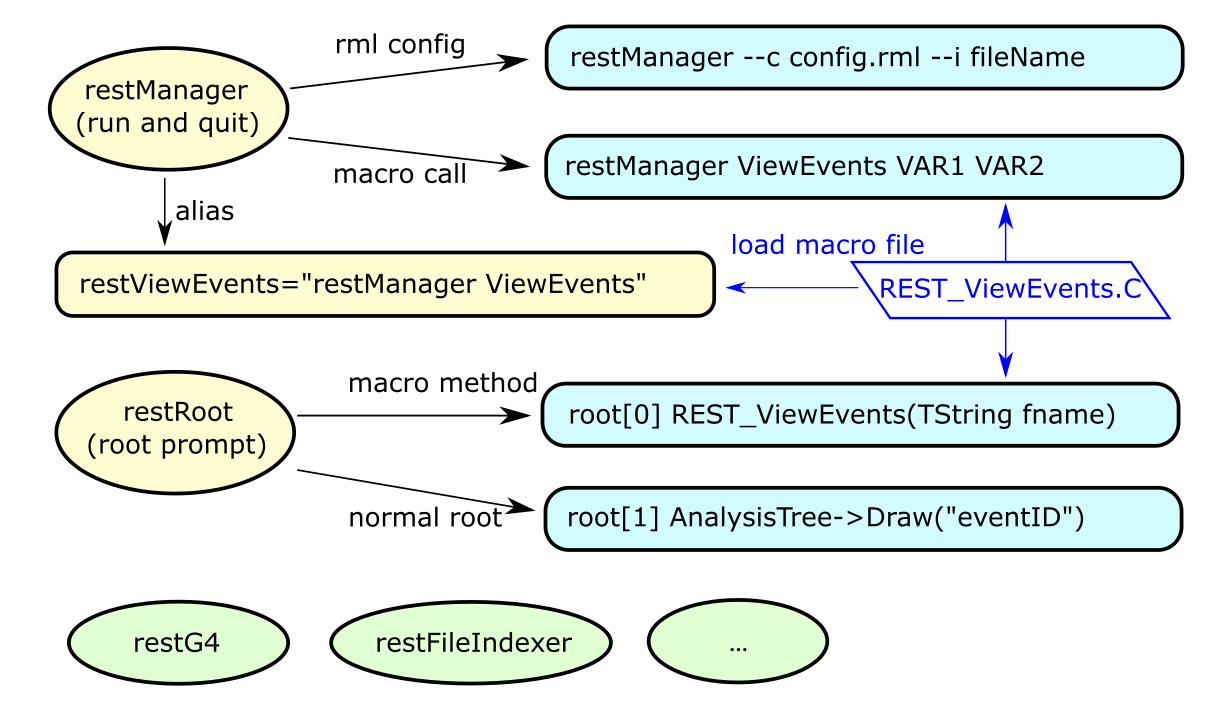
\includegraphics[width=0.9\linewidth]{images/executables.png}}
	\caption{REST executables running logic. \emph{restManager} and \emph{restRoot} work together to provide full access to the REST framework functionalities. Pre-defined ROOT C++ macro files are accessible through different interfaces, as it is shown through the \emph{REST\_ViewEvents.C} macro. Applications based on REST framework (green bubbles) extend the scope of the framework by providing additional functionalities, such as \emph{restG4} or \emph{restFileIndexer}.}
	\label{fig:executables}
\end{figure}

A bash script, \emph{rest-config}, is generated at each project compilation to provide information on the configuration of a particular build and to facilitate the linking of REST with external applications. It is important to remark that once REST has been compiled with a particular version of ROOT, Geant4 or Garfield, that compilation of REST must only be used with those versions. The shell script \emph{thisREST.sh} will be responsible to load the ROOT, Geant4, Garfield, or any other packages required, so that they match the correct versions used to compile REST at runtime.

\subsection{Project structure, versioning and code validation}
% submodule strategy

The main framework defines the basic functions, and describes the behavior of the main elements of REST. As previously mentioned, it also serves to centralize all the REST-for-Physics components, such as packages or libraries, and eventually dedicated projects. We have adopted a \emph{git submodule}\footnote{From this point we introduce a few concepts connected with the code versioning system, \emph{git}, that are broadly available online, such as \emph{commit} or \emph{submodule}. When we refer to those alien concepts we will highlight them using the \emph{git} keyword followed by the specific concept name.} strategy to integrate those components in a modular way inside the main framework repository. This scheme allows to independently monitor the development activity at each of those components, to isolate technical issues, and to focus on their functionality. Each component evolves independently with its own version or tracking system. A particular state of the code at each of those components is fixed at the main framework through a \emph{git commit} hash, or unique number. When that happens, the corresponding \emph{git commit} becomes the official component version of REST.

The framework repository fully centralizes the versioning system of REST, understood as the state of the code at a given period of time, including the state of the official \emph{git submodules} attached to it. Any REST \emph{metadata} object written to disk using the ROOT I/O scheme will be stamped with metadata values that ensure that the data written to disk has been processed with a given version, or state of the code. In order to certify that, two of those metadata members will be initialized at the code compilation time. The first metadata member will guarantee the source code was built from a clean, unmodified state with respect to the \emph{git remote} repository, and the second metadata member will certify that the corresponding framework code state is associated with an official \emph{git tag} release, where each \emph{git tag} generated at the main framework repository will automatically produce a code release referenced and citable at the Zenodo system\,\cite{javier_galan_2021_5092550}.

On top of that versioning strategy, it is important to mention that REST properly implements the ROOT schema evolution and ensures backwards compatibility for objects that have suffered changes in their data members.

%Those libraries and packages are kept as \emph{git submodules} of REST main framework, with their versions evolving independently. Therefore, the development of \emph{sub-modules} could be separated from the main framework, contributing to a series of git repositories under multi-person work. During installation, specific libraries for different workloads can be selected to download, compile and install.

% no need to explain TRestTask since it doesn't bring new concept

% \subsection{Basic tools}
% versioning strategy
% pipeline  validation

To ensure the code quality and stability with time, each repository integrates a validation pipeline where basic tests on the code are performed: some examples are code formatting and style validation, testing the proper libraries integration and building of executable programs or, even more important, testing basic results from complex data processing chains (see Figure\,\ref{fig:pipelines}). Each modification to the code, or \emph{git commit}, will be verified by running those validation pipelines. If a modification to the code produces an unexpected value on a consolidated data processing routine, the contributor will be notified, and changes will only become official after peer reviewing the code. This fact is extremely relevant to guarantee that the algorithms keep producing the expected results, or in the undesired case of a bug code identification, promptly identify the affected routines after its correction. Moreover, validation pipelines might serve as running examples to show the integration or use of a specific tool or element operating inside the framework.

\begin{figure}[h]
  \centering
  \raisebox{-0.5\height}{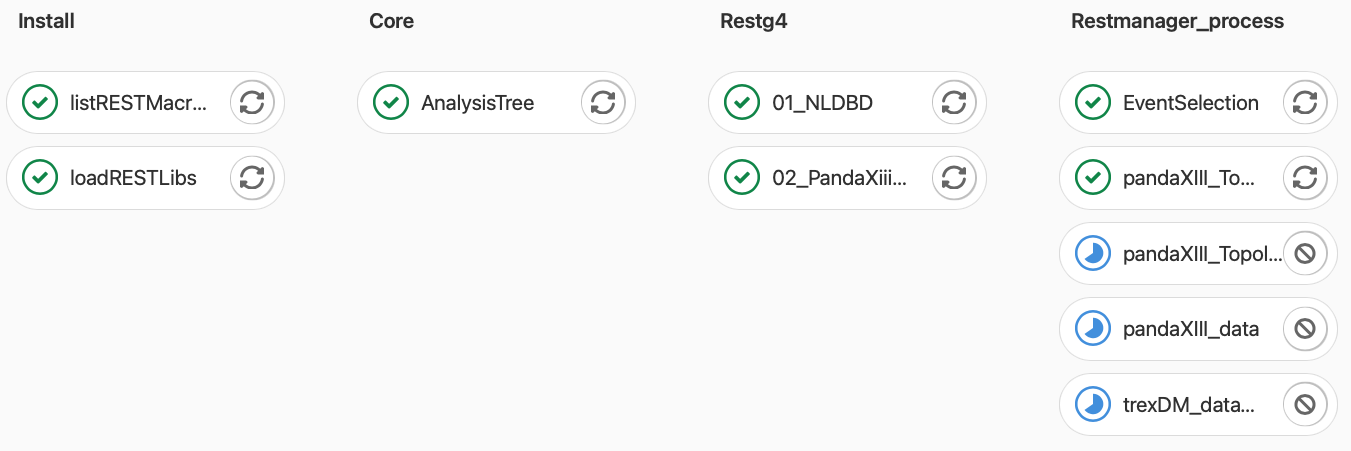
\includegraphics[width=0.95\linewidth]{images/pipelines3.png}}
	\caption{A snapshot from a validation pipeline at \emph{gitlab.cern.ch} running different tests triggered by an update to the code at the main framework repository. We observe different validation stages, from the most basic tests on the left, including compilation and installation to complex data chain processing tests on the right.}\label{fig:pipelines}
\end{figure}
